\documentclass[12pt,a4paper]{article}

% Paquetes de configuración del documento
\usepackage[utf8]{inputenc}
\usepackage[spanish]{babel}
\usepackage[T1]{fontenc}
\usepackage[margin=2.5cm]{geometry}
\usepackage{fancyhdr}
\usepackage{tabularx}
\usepackage{array}
\usepackage{siunitx}
\sisetup{per-mode=symbol}
\usepackage{csquotes}
%Paquetes para simbologia%
\usepackage{amsmath}
\usepackage{amsfonts}
\usepackage{amssymb}
\usepackage{physics}
\usepackage{longtable}
\usepackage{graphicx}
\usepackage{caption}
\usepackage{float}
\usepackage{xurl}
\usepackage[colorlinks=true,
            linkcolor=black,
            urlcolor=myblue,
            citecolor=black,
            filecolor=black]{hyperref}
 % Opción estándar para enlaces
\Urlmuskip=0mu plus 1mu          % Mejora el espaciado para permitir cortes
\usepackage{subcaption}  % en el preámbulo
\usepackage{pgfplots}
\pgfplotsset{compat=1.18}
\usepackage{tikz}
\usepackage{xcolor}
\definecolor{myblue}{RGB}{42, 127, 179}

\pagestyle{fancy}
\chead{\textit{Materiales Metálicos}}
\rhead{\textit{UTN-FRVM}}
\lhead{\textit{Ingeniería Mecánica}}

\begin{document}
\begin{titlepage}
	
	\begin{center}
		{\huge \textit{Universidad Tecnológica Nacional}}\\
        \vspace{0.5cm}
		{\LARGE \textit{Facultad Regional Villa María}}\\
		\vspace{1.5cm}
        {\LARGE{\textit{Ingeniería Mecánica - Materiales Metálicos}}}\\
		\vspace{1.5cm}
        \LARGE{\textit{Trabajo Práctico 3-06}}
	\end{center}
	
	\vfill

    \textit{Grupo DEL RÍO:}
	\begin{itemize}
		\item \textit{Abregú, Iván.}
		\item \textit{Antico, Rodrigo.}
		\item \textit{Brussa,Julián.}
		\item \textit{Cabral, Franco.}
        \item \textit{Cárdenas, Felipe.}
        \item \textit{Cardozo, Martín.}
        \item \textit{Córdoba, Nathan.}
        \item \textit{Cucco, Ramiro.}
        \item \textit{del Río, Juan.}
        \item \textit{Guerini, Nazareno.}
        \item \textit{Medina, Ivo.}
        \item \textit{Ortiz, Gastón.}
        \item \textit{Picos, Elías.}
        \item \textit{Quinteros, Lautaro.}
	\end{itemize}
    
	\textit{Docentes:}
	\begin{itemize}
		\item \textit{Dr. Lucioni, Eldo José.}
		\item \textit{Ing. Victorio Vallaro, Juan Manuel.}
	\end{itemize}
	\centering
	\today
	
\end{titlepage}

\newpage
\tableofcontents

\begin{abstract}
    \textbf{Desarrollar conceptualmente el interrogante: ¿Qué es la selección de materiales?}

    \underline{INFORMACIÓN ADICIONAL:}
    \begin{itemize}
        \item Michael Farries Ashby - Biografía. Sitio Web: \url{https://en.wikipedia.org/wiki/Michael_F._Ashby}.
        \item \url{https://www.upm.es/sfs/Rectorado/Gabinete%20del%20Rector/Honoris%20Causa/curriculum/Doctor%20Honoris%20Causa%20Michael%20Ashby.pdf} \{MM-CAD-IA U1\}
    \end{itemize}
\end{abstract}

\section{Desarrollo conceptual.}
\subsection{¿Qué es la selección de materiales?}

Para poder responder esta interrogante, podríamos primero considerar que ante 
cualquier proyecto surgen 3 interrogantes: 
\paragraph{¿Qué hago?, ¿Cómo lo hago?} Cuando ya se ha definido cuales son las prestaciones que debe de tener cualquier dispositivo, a la vez que se consagra un diseño el cual se adapte a las posibilidades físicas del proyecto y a su entorno de trabajo, solo quedaría definir el último interrogante.
\paragraph{¿Con qué lo hago?} Siguiendo con esta lógica nosotros sabríamos bajo qué condiciones trabajará el proyecto, cuáles son las aptitudes a poseer y los defectos permisibles. Por Ej: no es necesario que nuestro producto resista la corrosión de los ácidos si no estará expuesto a dicha situación. 

Según el material de estudio propuesto por la cátedra sobre selección de materiales (Verdeja, L.F.  Elección y selección de materiales estructurales en ingeniería) podríamos basarnos principalmente en algunas relaciones entre propiedades, \(E/\rho\); \(\sigma_y/\rho\); \(K_c/\rho\); etc.

Se puede entender rápidamente que la densidad es de gran interés a la hora de seleccionar un material, esto es algo completamente lógico, pues no se podrían construir aviones, helicópteros,  naves espaciales, ni ningún medio de transporte de vuelo, si el peso de dicho transporte le impide volar. Así es que la relación entre la masa de un objeto y su volumen, es tan importante, por otro lado el saber cuánta masa de un material tengo, me ndica la cantidad de ese material que poseo y por consecuencia puedo relacionar mi diseño con su propio costo de forma rápida.
De todos modos no solo no debemos de guiar por las propiedades mecánicas, en un contexto donde sería de sumo interés el comportamiento diamagnético descartaríamos rápidamente la mayoría de los metales y nuestro foco acabaría en las demás familias de materiales, según Ashby, las familias son las dispuestas como en la \autoref{fig:familias}.

\begin{figure}[t]
    \centering
    \begin{subfigure}{0.45\textwidth}
        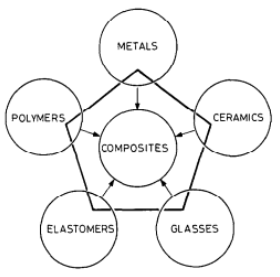
\includegraphics[width=\textwidth]{Figuras/image.png}
        \subcaption{Las distintas familias de materiales.}
        \label{fig:familias}
    \end{subfigure}
    \begin{subfigure}{0.45\textwidth}
        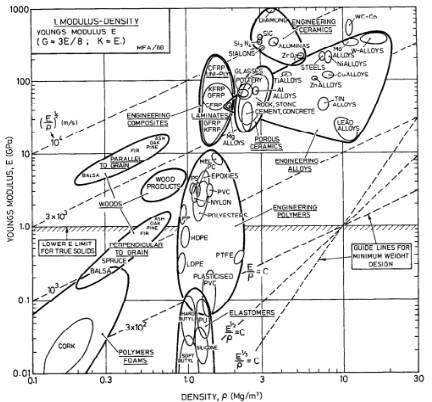
\includegraphics[width=\textwidth]{Figuras/grafico.png}
        \caption{Método gráfico para la selección de materiales.}
        \label{fig:grafico}
    \end{subfigure}    
\end{figure}

También se encargó de relacionar cada uno de estos en función de sus relaciones \(E/\rho\) y plasmarlo en una gráfica (Método Gráfico) como se encuentra en la \autoref{fig:grafico}.

Además del método gráfico, podemos considerar otros tipos de metodologías para la correcta selección de un material, lo importante es que el ingeniero sea capaz de manejar todos estos métodos para de esta manera lograr una selección eficaz. Entre estos tipos encontramos:

El \textbf{método tradicional:} se basa en la experiencia y en la selección de materiales análogos con un historial de buen desempeño en aplicaciones similares. No obstante, presenta limitaciones al no considerar siempre las nuevas tecnologías, los materiales avanzados o un análisis exhaustivo de las condiciones específicas de servicio.

\textbf{Metodología basada en bases de datos:} en internet se dispone de una extensa variedad de bases de datos de materiales, disponibles en acceso abierto o comercializadas por proveedores especializados. Estas bases de datos son el resultado de investigaciones y ensayos exhaustivos. Se clasifican principalmente en dos categorías: numéricas y bibliográficas. Entre las más relevantes destacan las bases de datos de ASTM, SAE, ASM, AISI y NASA, entre otras. En los últimos años ganó popularidad una base de datos pública llamada Matweb (sitio web: \url{https://matweb.com/}), que resalta por tener una amplia variedad de materiales.

Mismo procedimiento que efectúa con otras propiedades relacionadas entre ellas incluso realizando gráficos para los diferentes tipos de productos interfamiliares, por ej: la relación entre la temperatura de transición vítrea de los plásticos y su resistencia a la tracción o la conductividad térmica y la difusividad de los metales.

\section{Conclusión.}

La selección de materiales, podría ser la capacidad de tomar la decisión más acertada a la hora de elegir con qué material construir un producto ya diseñado, evaluando y teniendo en cuenta todo el panorama de posibilidades. Para ello evidentemente quien decida dicho material debe ser alguien capacitado y conocedor de la amplia gama de materiales existentes y de cómo se comportan. Debe utilizar alguno de los diferentes tipos de métodos de elección de materiales como el método tradicional,método con ayuda de bases de datos, método gráfico, estos métodos permiten una selección más eficiente y adecuada de materiales en comparación con una elección sin análisis estructurado, reduciendo riesgos de fallos y optimizando costos y desempeño.

\section{Bibliografía.}
\begin{itemize}
    \item González, H.A. y Mesa, D.H. La importancia del método en la selección de materiales. Scientia et Technica Año X, No 24, Mayo 2004. UTP. ISSN 0122-1701. (pp.175-180) \{MM-CAD-1.2\}.
    \item Verdeja, L.F.  Elección y selección de materiales estructurales en ingeniería. RDM Revista de Minas. Año 1993, Número 8.  (pp. 47-57) \{MM-CAD-1.2\}.
    \item Michael Farries Ashby - Biografía. Sitio Web: \url{https://en.wikipedia.org/wiki/Michael_F._Ashby}.
    \item \url{https://www.upm.es/sfs/Rectorado/Gabinete%20del%20Rector/Honoris%20Causa/curriculum/Doctor%20Honoris%20Causa%20Michael%20Ashby.pdf} \{MM-CAD-IA U1\}
\end{itemize}

\end{document}